%-------------------------------------------------------------------------
\subsection{Kueper problem}
\subsubsection*{Background}
Both primary variable schemes are now further tested with a benchmark chosen to test two-phase flow in heterogeneous media. Kueper and Frind (1991) developed a model to simulate their experiment for DNAPL penetration (Kueper et al., $1989$). The simultaneous movement of a dense non-wetting phase (DNAPL) through an initially wetting phase (water) saturated heterogeneous porous media may be represented mathematically as a case of two-phase flow. A distinctive feature of the solution is that the primary variables solved for, wetting phase pressure and wetting phase saturation, are both existent throughout the solution domain regardless of whether the non-wetting phase is present.


The continuity equation of each phase ($\gamma$) can be defined by
\begin{equation}
\frac{\partial (n {\rho}^{\gamma} S^{\gamma})}{\partial t} + \nabla \cdot ({\rho}^{\gamma} \mathbf{q}^{\gamma}) = \mathbf{Q}^{\gamma}, \gamma=w, nw
\label{eq:mcwtMassEq}
\end{equation}
where $n$ is porosity, $S^{\gamma}$ is saturation, $\rho^{\gamma}$ is density, $\mathbf{Q}^{\gamma}$ is a source or sink term, and $\mathbf{q}^{\gamma}$ is the Darcy velocity for phase $\gamma$ defined by
\begin{equation}
\mathbf{q}^{\gamma}=-{\mathbf K} \frac{\kappa_r^{\gamma}}{\mu^{\gamma}}(\nabla p^{\gamma}-{\rho}^{\gamma} \mathbf{g}), \gamma=w, nw
\label{eq:mcwtFluxEq}
\end{equation}

where $\kappa_r^{\gamma}$ is relative permeability, $\mu^{\gamma}$ is viscosity, $p^{\gamma}$ is pressure for phase $\gamma$, $\textbf{K}$ is intrinsic permeability tensor and $\mathbf{g}$ is the gravitational vector.  

Inherently for saturation, the sum of all saturation in pore space is
\begin{equation}
{\sum S^{\gamma}}=1
\label{eq:mcwtFluxEq}
\end{equation}

Assuming relative preference (i.e., wettability) of the fluid to media exists and it is not negligible, the capillary pressures relation for a two-phase system is defined over representative elementary volume (REV) by 

\begin{equation}
p_c=p_{nw}-p_w
\label{eq:mcwtFluxEq}
\end{equation}                                                 
where $p_c$ is capillary pressure, $p_{nw}$ is pressure for the non-wetting phase fluid and $p_w$ is the wetting phase fluid. 

\begin{figure}[!htb]
\begin{center}
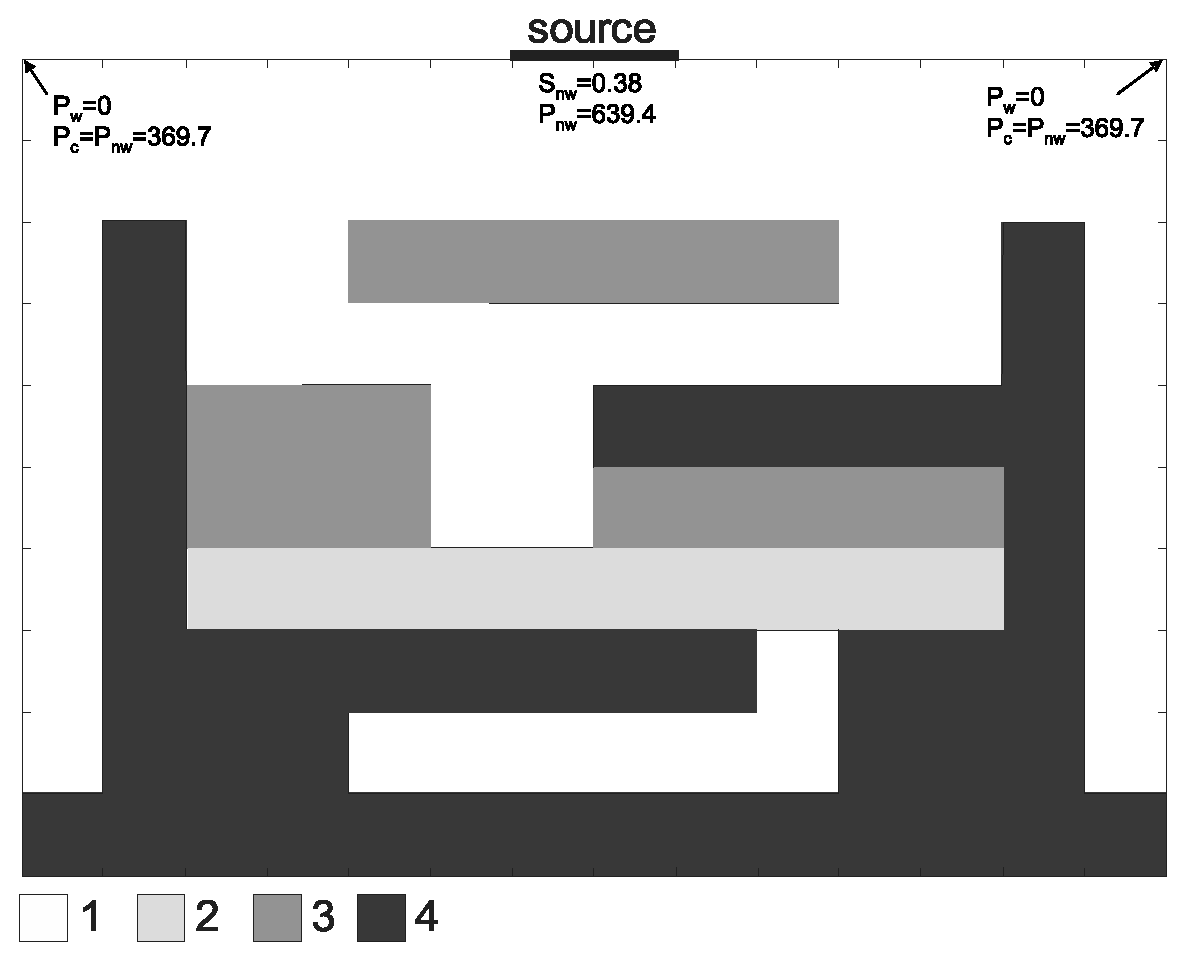
\includegraphics[height=5cm]{chapter_14/figures/KueperConfiguration.eps}
\end{center}
\caption{Configuration of heterogeneous media in parallel-plate cell.}
\label{mcwt:keuperconfig}
\end{figure}

\subsubsection*{Definition}
A $60cm\times80cm\times0.6cm$ parallel-plate glass-lined cell was packed with four types of sands and initially fully saturated with water. The configuration of the assembled sand lenses and the two sets of the boundary conditions for the $p_w-S_{nw}$ and $p_c-p_{nw}$ schemes are illustrated in Fig. \ref{mcwt:keuperconfig}. Concerning to the constitutive relation between relative permeability and saturation and capillary pressure and saturation, they have used the Brooks-Corey model. 

Properties of Sands for the Brooks-Corey model are measured experimentally and summarized in the following tables. The numerical solutions obtained from the $p_w-S_{nw}$ scheme and the $p_c-p_{nw}$ scheme for the benchmark Kueper and Frind ($1991$) are compared against each other in Fig. \ref{mcwt:keuperresults}. 

\begin{table}[!htb]
\begin{center}
\begin{tabular}{|l|l|l|l|}
\hline
Fluid properties & Unit & Wetting fluid	& Non-wetting fluid \\
\hline
Density &	$kg.m^{-3}$ &	$1.0\times10^3$ &	$1.0\times10^3$ \\ 
\hline
Viscosity &	$Pa\cdots$ & $1.0\times10^{-3}$ &	$1.0\times10^{-3}$ \\
\hline
Residual saturation &	- &	0.0 &	0.0 \\
\hline
Maximum saturation &	- &	1.0 &	1.0 \\
\hline
\end{tabular}
\caption{Fluid and medium properties.}
\end{center}
\end{table}

\begin{table}[!htb]
\begin{center}
\begin{tabular}{|l|l|l|}
\hline
Medium properties & Unit & Medium\\
\hline
$\Delta x$ & m &	0.01 \\
\hline
$\Delta t$ & s &	100 \\
\hline
Porosity & - &	0.3 \\
\hline
Intrinsic permeability & $m^2$ & $1\times10^{-10}$ \\
\hline
Brook-Corey's index &	- &	2 \\
\hline
Entry pressure & Pa & $5\times10^3$ \\
\hline
\end{tabular}
\caption{Space and time discretization.}
\end{center}
\end{table}

\begin{table}[!htb]
\begin{center}
\begin{tabular}{|l|l|l|l|l|l|}
\hline
Property & $P_d$(Pa) & $\lambda$(-) &	$S_{wr}$(-) &	k($m^2$) &	$n$(-) \\
\hline
1	& 369.73 & 3.86	& 0.078	& $5.04\times10^{-10}$ & 0.40 \\ 
\hline
2	& 434.45 & 3.51 & 0.069 &	$2.05\times10^{-10}$ & 0.39 \\
\hline
3	& 1323.95 &	2.49 & 0.098 &	$5.26\times10^{-11}$ & 0.39 \\
\hline
4	& 3246.15	& 3.30 & 0.189 & $8.19\times10^{-12}$ &	0.41 \\
\hline
\end{tabular}
\caption{Hydraulic properties of sands for the Brooks-Corey model.}
\end{center}
\end{table}

\subsubsection*{Results}
Both schemes produce DNAPL plume propagation physically until the plume reaches the less permeable media under the top medium in the model domain. The striking difference occurs at the interface between these two media. While the pwSnw scheme simulates the plume to infiltrate into the less previous medium, the $p_c-p_{nw}$ scheme forces the plume to bypass the less previous medium. A similar experiment and simulation comparison against experimental observation are also conducted by Helming and Huber ($1998$). They have reported unphysical fluid behavior captured by the $p_w-S_{nw}$ scheme, a phenomenon that can be avoided with fully upwind technique (Helming and Huber, $1998$). 

\begin{figure}[!htb]
\begin{center}
\includegraphics[height=12cm]{chapter_14/figures/Kueper.eps}
\end{center}
\caption{Comparison of the results obtained from the $p_w-S_{nw}$ and $p_c-p_{nw}$ schemes. The second column shows good agreement with observed distribution of DNAPL of the experiment (Kueper and Frind $1991$).}
\label{mcwt:keuperresults}
\end{figure}